\chapter{Input and Output}\label{input-output}

{\LARGE IO} is of very importance for software testing
and business development. There are two parts to it, the generic IO, 
which deals with how to read/write from disk, and to and from url.
There is another part of the data stuff, that is structured data.
nJexl let's you do both, and those are the topic of this chapter.

\begin{section}{Reading}

\begin{subsection}{read() function}
Reading is done by this versatile $read()$ function.
\index{read()}
The general syntax is :
\begin{lstlisting}[style=JexlStyle]
value = read(source_to_read)
\end{lstlisting}
The source can actually be a file, an UNC path, an url.
Note that given it is a file, $read()$ reads the whole 
of it at a single go, so, be careful with the file size. 

\begin{lstlisting}[style=JexlStyle]
value = read('my_file.txt')
/* value contains all the text in my_file.txt */
\end{lstlisting}
\end{subsection}

\begin{subsection}{Reading from url : HTTP GET}
\index{read() : http get}
Read can be used to read from an url.
Simply :

\begin{lstlisting}[style=JexlStyle]
value = read('http://www.google.co.in')
/* value contains all the data in the google home page */
\end{lstlisting}

To handle the timeouts, it comes with overloads:
\index{read() : url timeout }
\begin{center}\begin{minipage}{\linewidth}
\begin{lstlisting}[style=JexlStyle]
// url, connection timeout, read timeout, all in millisec
value = read('http://www.google.co.in', 10000, 10000 )
/* value contains all the data in the google home page */
\end{lstlisting}
\end{minipage}\end{center}

\index{read() : http get : url generation }
To generate the url to $get$, the fold function comes handy:
\begin{lstlisting}[style=JexlStyle]
_url_ = 'https://httpbin.org/get'
params = { 'foo' : 'bar' , 'complexity' : 'sucks'  }
// str: is the namespace alias for 'java.lang.String'
data = str{  
          str:format( "%s=%s" , $.key, $.value )  
      }( params.entrySet() , '&' )
response = read( str:format("%s?%s", _url_ , data ) )
\end{lstlisting}
\index{restful api : get}
And that is how you do a restful api call, using $get$.
\end{subsection}

\begin{subsection}{Reading All Lines}
\index{ lines() }
The function $lines()$ reads all the lines, 
and puts them into different strings, so that it returns 
a list of strings, each string a line.
With no other arguments, it defers the reading of next line, 
so it does not read the whole bunch together.

\begin{lstlisting}[style=JexlStyle]
for ( line : lines('my_file.txt') ){
   write(line) // proverbial cat program 
}
\end{lstlisting}
In short, the $lines()$ method yields an iterator.
But with this, it reads the whole file together :

\begin{lstlisting}[style=JexlStyle]
ll = lines ( 'my_file.txt' , true )
\end{lstlisting}

This is again a synchronous call, and thus, it would 
be advisable to take care.

\end{subsection}

\end{section}

\begin{section}{Writing}

\begin{subsection}{write() or print() function}

We are already familiar with the write function.
\index{write()}\index{print()}
With a single argument, it writes the data back to the standard output.
The function is aliased as \emph{print()} which is same as \emph{write()}:
\begin{lstlisting}[style=JexlStyle]
write('Hello,World!') ; print('Hello,World!') ; 
\end{lstlisting}

Given that the first argument does not contain a "\%" symbol,
the write functionality also writes the whole string to a file
with the name :
\index{write() : file }
\begin{lstlisting}[style=JexlStyle]
// creates my_file.txt, writes the string to it 
write('my_file.txt', 'Hello,World!')
\end{lstlisting}

Given there is formatting arguments with "\%" symbols, 
works as if it is a $printf()$ call :
\index{write() : formatting}
\begin{lstlisting}[style=JexlStyle]
//  writes the string to it 
write('%s\n', 'Hello,World!')
\end{lstlisting}
The formatting guide can be found 
\href{https://sharkysoft.com/archive/printf/docs/javadocs/lava/clib/stdio/doc-files/specification.htm}{here}. 
\end{subsection}

\begin{subsection}{Writing to url : HTTP POST}
Write can be used to send POST call to urls, observe the following:
\index{write() : url : post}
\begin{lstlisting}[style=JexlStyle]
_url_ = 'https://httpbin.org/post'
params = { 'foo' : 'bar' , 'complexity' : 'sucks'  }
response = write(  _url_ , params )
\end{lstlisting}
\end{subsection}

\begin{subsection}{Sending to url : send() function}
\index{send()}
To write back to url, or rather for sending anything to a server,
there is a specialised send() function.

\begin{lstlisting}[style=JexlStyle]
_url_ = 'https://httpbin.org/post'
params = { 'foo' : 'bar' , 'complexity' : 'sucks'  }
// url,  protocol     ,  body, headers, connection timeout, read timeout  
response = send(  _url_ , "GET"  , params , {:} , 1000, 1000 )
\end{lstlisting}

The SOAP XML stuff can be easily done with $send$.
See the example soap body we  will send to :

\begin{lstlisting}[style=xmlStyle]
<?xml version="1.0" encoding="utf-8"?>
<soap:Envelope xmlns:xsi="http://www.w3.org/2001/XMLSchema-instance" 
	xmlns:xsd="http://www.w3.org/2001/XMLSchema" 
	xmlns:soap="http://schemas.xmlsoap.org/soap/envelope/">
    <soap:Body>
        <GetWeather xmlns="http://www.webserviceX.NET">
            <CityName>%s</CityName>
            <CountryName>%s</CountryName>
        </GetWeather>
    </soap:Body>
</soap:Envelope>
\end{lstlisting}

And this is how we $send$ the SOAP: \index{SOAP}

\begin{center}\begin{minipage}{\linewidth}
\begin{lstlisting}[style=JexlStyle]
template_pay_load = read('samples/soap_body.xml')
pay_load = str:format ( template_pay_load , 
                     'Hyderabad', 'India' )
headers = { "SOAPAction" : "http://www.webserviceX.NET/GetWeather" , 
             "Content-Type" : "text/xml; charset=utf-8" }
__url__ = "http://www.webservicex.net/globalweather.asmx"
resp = send( __url__ , "POST" , pay_load , headers ) 
x = xml(resp)
sr = x.element("//GetWeatherResult")
write(sr.text)
\end{lstlisting}
\end{minipage}\end{center}

\end{subsection}

\end{section}

\begin{section}{File Processing}
We talked about a bit of file processing in $read$ and $write$.
But if we want to read a file line by line, then we have to use something else.

\begin{subsection}{lines() function}
\index{lines()} 
lines() function generates an iterator, which can be used to read the file.
It caches the previous reads, so after you ended reading, resetting the iterator 
you can read it again. Observe we are replicating the Unix program wc: \index{wc : word count}

\begin{center}\begin{minipage}{\linewidth}
\begin{lstlisting}[style=JexlStyle]
fi = lines('my_file.txt' )
// count no of lines 
lc = lfold{ _$_ += 1 }(fi,0)
// resets the iterator
fi.reset()
// character count 
cc = lfold{ _$_ += size($) + 1  }(fi,0)
// resets the iterator
fi.reset()
// word count?
wc = lfold{ _$_ += size($.split(" \t") ) }(fi,0)
// reset again 
fi.reset()
// or in a single go, using a tuple value 
#(l,w,c) = lfold{ 
               // do a tuple assignment 
               #(lc,cc,wc) = _$_ 
               lc+=1 ; cc += size($) + 1  
               wc += size($.split(" \t") )
              _$_ = [ lc, cc, wc ] 
      }(fi,[0,0,0] )
\end{lstlisting}
\end{minipage}\end{center}

\end{subsection}

\begin{subsection}{fopen() function}
\index{fopen()}
In some rare scenarios, to write optimal code, 
one may choose to read, write, append on files.
The idea is then, using $fopen()$ function.
The syntax is :

\begin{lstlisting}[style=JexlStyle]
fp = fopen( path [, mode_string ] )
\end{lstlisting}

The mode strings are defined as such:
\index{fopen() : open modes}
There are 3 modes :
\begin{enumerate}
\item{ Read : the default mode : specified by "r" }
\item{ Write : the write mode : specified by "w"  }
\item{ Append : the append mode : specified by "a" }
\end{enumerate}

\end{subsection}

\begin{subsection}{Reading}
\index{fopen() : reading}
To read, one must open the file in read mode.
This returns a java \href{https://docs.oracle.com/javase/8/docs/api/java/io/BufferedReader.html}{BufferedReader} object.
Now, something like \href{https://docs.oracle.com/javase/8/docs/api/java/io/BufferedReader.html#readLine--}{readLine}
can be called to read the file line by line, in a traditional way to implement the $cat$ command : \index{cat}

\begin{center}\begin{minipage}{\linewidth}
\begin{lstlisting}[style=JexlStyle]
// open in read mode : get a reader
fp = fopen( path ,"r" )
while ( true ){
   // call the standard java functions
   line = fp.readLine()
   break( null == line )
   write(line)
}
// close the reader
fp.close()
\end{lstlisting}
\end{minipage}\end{center}

\end{subsection}

\begin{subsection}{Writing}
\index{fopen() : writing}

To write, one must open the file in write or append mode.
This returns a java \href{https://docs.oracle.com/javase/8/docs/api/java/io/PrintStream.html}{PrintStream} object.
Now, something like \href{https://docs.oracle.com/javase/8/docs/api/java/io/PrintStream.html#println-java.lang.Object-}{println()}
can be called to write to the file :

\begin{lstlisting}[style=JexlStyle]
// open in read mode : get a reader
fp = fopen( "hi.txt" ,"w" )
// call the standard java functions
fp.println("Hi")
// close the Stream
fp.close()
\end{lstlisting}

\end{subsection}

\end{section}

\begin{section}{Working with JSON}

\begin{subsection}{What is JSON?}
\index{json}
JSON is being defined formally in \href{http://www.json.org}{here}.
The idea behind JSON stems from : \emph{JavaScript Object Notation}.
There are many ways to define an object, one of them is very practical :
\begin{center}
\emph{Objects are property buckets.}
\end{center}

That definition ensures that the ordering layout of the properties does not matter at all.
Clearly :
$$
\{  ``x'' : 10 , ``y'' : 42 \} == \{  ``y'' : 42 , ``x'' : 10 \}
$$
Thus, we reach the evident conclusion, JSON are nothing but Dictionaries.
Hence in nJexl they are always casted back to a dictionary.

\end{subsection}

\begin{subsection}{json() function}
Suppose the json string is there in a file:

\begin{lstlisting}[style=JexlStyle]
/* sample.json file  */
{
  "noga": {
    "dbName": "noga",
    "url": "jdbc:postgresql://localhost:5432/noga",
    "driverClass" : "org.postgresql.Driver",
    "user": "noga",
    "pass": ""
  },
  "some2": {
    "dbName": "dummy",
    "url": "dummy",
    "driverClass" : "class",
    "user": "u",
    "pass": "p"
  },
}
\end{lstlisting}
To read the file ( or the text which has json) :
\begin{lstlisting}[style=JexlStyle]
jo = json('sample.json')
\end{lstlisting}
The $json()$ function can read also from the string argument.
The return result object is either a Dictionary object, 
or an array object, based on what sort of json structure was passed.
\end{subsection}

\begin{subsection}{Accessing Fields}
Now, to access any field:
\begin{lstlisting}[style=JexlStyle]
jo.noga.dbName // "noga"
jo.some2.driverClass // "class" 
\end{lstlisting}
In effect, one can imagine this is nothing but a big property bucket.
For some, there is this thing called \href{http://goessner.net/articles/JsonPath/}{JSONPath}, \index{JSONPath}
which is clearly not implemented in nJexl, because that is not a standard.
In any case, given json is a string, to check whether a text exists or not is a regular string search.
Given whether a particular value is in the hierarchy of the things or not, 
that is where the stuff gets interesting. 

For parameterised access, Currying is a better choice:

\begin{lstlisting}[style=JexlStyle]
prop_value = 'noga.dbName'  
value = `jo.#{prop_value}` // same thing, "noga"
\end{lstlisting}
In this way, one can remove the hard coding of accessing JSON objects.
\end{subsection}

\end{section}

\begin{section}{Working with XML}
\index{xml}

Please, do not work with xml. 
There are many reasons why xml is a \href{http://harmful.cat-v.org/software/xml}{terrible idea}.
The best of course is :
\begin{center}
\emph{
XML combines the efficiency of text files with the readability of binary files
 -- unknown
 }
\end{center}

But thanks to many big enterprise companies - it became a norm to abused human intellect - the last are obviously Java EE usage in Hibernate, Springs and Struts. Notwithstanding the complexity and loss of precise network bandwidth - it is a very popular format. 
Thus - against my better judgment I could not avoid XML.

\begin{subsection}{xml() function}
\index{xml()}

Suppose, we have an xml in a file sample.xml :
\begin{lstlisting}[style=xmlStyle]
<slideshow 
title="Sample Slide Show"
date="Date of publication"
author="Yours Truly" >
<!-- TITLE SLIDE -->
<slide type="all">
  <title>Wake up to WonderWidgets!</title>
</slide>
<!-- OVERVIEW -->
<slide type="all">
    <title>Overview</title>
    <item>Why <em>WonderWidgets</em> are great</item>
    <item/>
    <item>Who <em>buys</em> WonderWidgets</item>
</slide>
</slideshow>
\end{lstlisting}
Call $xml()$ To load the xml file ( or a string ) into an 
\href{https://github.com/nmondal/njexl/blob/master/lang/src/main/java/com/noga/njexl/lang/extension/dataaccess/XmlMap.java}{XmlMap} object :
\begin{lstlisting}[style=JexlStyle]
x = xml('sample.xml', 'UTF-8' ) // x is an XmlMap object
\end{lstlisting}
The encoding string ( UTF-8 ) is optional. 
Default is UTF-8. \index{xml : encoding}

The function xml() can also convert a proper Java Object into string, 
in other words, it does \href{https://msdn.microsoft.com/en-us/library/182eeyhh(v=vs.110).aspx}{Xml Serialisation}. 
Suppose we have the JSON object : \index{xml: serialisation}

\begin{center}\begin{minipage}{\linewidth}
\begin{lstlisting}[style=JexlStyle]
/* demo.json file  */
{
    "glossary": {
        "title": "example glossary",
        "GlossDiv": {
            "title": "S",
            "GlossList": {
                "GlossEntry": {
                    "ID": "SGML",
                    "SortAs": "SGML",
                    "GlossTerm": "Standard Generalized Markup Language",
                    "Acronym": "SGML",
                    "Abbrev": "ISO 8879:1986",
                    "GlossDef": {
          "para": "A meta-markup language, used to create markup languages such as DocBook.",
          "GlossSeeAlso": ["GML", "XML"]
                    },
                    "GlossSee": "markup"
                }
            }
        }
    }
}
\end{lstlisting}
\end{minipage}\end{center}

This is how we can generate an XML out of it :

\begin{center}\begin{minipage}{\linewidth}
\begin{lstlisting}[style=JexlStyle]
// load json 
jo = json('db.json')
// convert to xml string 
x = xml(jo)
\end{lstlisting}
After formatting the xml string is :
\begin{lstlisting}[style=xmlStyle]
<root>
  <glossary>
    <title>example glossary</title>
    <GlossDiv>
      <GlossList>
        <GlossEntry>
          <GlossTerm>Standard Generalized Markup Language</GlossTerm>
          <GlossSee>markup</GlossSee>
          <SortAs>SGML</SortAs>
          <GlossDef>
                 <para>A meta-markup language, used to 
                 create markup languages such as DocBook.
                 </para>
            <GlossSeeAlso>
              <i>GML</i>
              <i>XML</i>
            </GlossSeeAlso>
          </GlossDef>
          <ID>SGML</ID>
          <Acronym>SGML</Acronym>
          <Abbrev>ISO 8879:1986</Abbrev>
        </GlossEntry>
      </GlossList>
      <title>S</title>
    </GlossDiv>
  </glossary>
</root>
\end{lstlisting}
\end{minipage}\end{center}

\end{subsection}

\begin{subsection}{Accessing Elements}
Given I have the XmlMap object, I should be able to find elements in it.
The elements can be accessed in two different ways.
\index{xml : pojo}
The first is, using the xml as a tree with $root$ and $children$.
That is easy, for example, for the previous json to xml generated :

\begin{lstlisting}[style=JexlStyle]
// XmlMap of the x 
y = xml(x)
y.root.children[0].name //glossary
y.root.children[0].children[0].text // example glossary 
\end{lstlisting}

For the slideshow xml: \index{xml : attribute}

\begin{center}\begin{minipage}{\linewidth}
\begin{lstlisting}[style=JexlStyle]
// XmlMap of the x 
x = xml('sample.xml') // slideshow xml 
x.root.name //slideshow
// access attributes 
x.root.children[0].attr.type // "all"
x.root.children[0].attr['type'] // "all"
\end{lstlisting}
\end{minipage}\end{center}

The other way of accessing elements, 
is to use the $element()$ function, 
which uses \href{https://en.wikipedia.org/wiki/XPath}{XPATH} :
\index{xml : element()}
\begin{lstlisting}[style=JexlStyle]
// XmlMap of the x 
x = xml('sample.xml') // slideshow xml 
// get one element  
e = x.element("//slide/title")// first title element 
e.text // "Wake up to WonderWidgets!"
e = x.element("//slide[2]/title" ) // second element 
e.text // "Overview"
\end{lstlisting}

In the same way, for selecting multiple elements, $elements()$
function is used : \index{xml : elements()}

\begin{lstlisting}[style=JexlStyle]
// XmlMap of the x 
x = xml('sample.xml') // slideshow xml 
// get all the elements called titles  
es = x.elements("//slide/title" ) // a list of elements 
// print all titles ?
lfold{  write( $.text ) }(es)
\end{lstlisting}

\end{subsection}

\begin{subsection}{XPATH Formulation}
\index{xml : xpath()}
For evaluation of xpath directly, there is $xpath()$ function 
defined. For example, to find the text of any element, 
one can use the following :

\begin{lstlisting}[style=JexlStyle]
// XmlMap of the x 
x = xml('sample.xml') // slideshow xml
// text of the title element 
s = x.xpath("//slide/title/text()" )  
\end{lstlisting}

For a list of all xpath functions see the specification in 
\href{https://www.w3.org/TR/xpath-functions-3}{w3c}.

To check if a condition exists or not, one can use the $exists()$ function.
\index{xml : exists()}
\begin{lstlisting}[style=JexlStyle]
// XmlMap of the x 
x = xml('sample.xml') // slideshow xml
// text of the title element, exists? 
b = x.exists("//slide/title/text()" ) // bool : true 
b = x.exists("//slide/title" ) // bool : true 
b = x.exists("//foobar" ) // bool : false 
\end{lstlisting}

Obviously, one can mix and match, that is, give a default to the $xpath()$ function :
\index{xml : xpath() default } 
\begin{lstlisting}[style=JexlStyle]
// string : text comes
t = x.xpath("//slide/title/text()" , 'NONE_EXISTS' )
// string : 'NONE_EXISTS'  
t = x.xpath("//foobar/text()",  'NONE_EXISTS' )  
\end{lstlisting}

\end{subsection}

\begin{subsection}{Xml to JSON}
\index{ xml : json() }
The xml can be converted to a suitable JSON equivalent, by invoking the $json()$ function.
This function is available on the XmlMap object, also the standard $json()$ function 
would convert any XmlMap object.

\begin{center}\begin{minipage}{\linewidth}
\begin{lstlisting}[style=JexlStyle]
// XmlMap of the x 
x = xml('sample.xml') // slideshow xml
// json form of the xml 
jo = x.json() 
jo = json(x)  // same as above
\end{lstlisting}
\end{minipage}\end{center}
 
\end{subsection}

\end{section}

\begin{section}{DataMatrix}
\index{DataMatrix}

A DataMatrix is an abstraction for a table with tuples of data as rows.
Formally, then a data matrix $M = (C,R) $ where $C$ a tuple of columns,
and $R$ a list of rows, such that  $\forall r_i \in R$ , $r_i$ is a tuple
of size $|r_i| = |C|$. In specificity, $r_i[C_j] \to r_{ij}$ , that is, 
the $i$'th rows $j$'th cell contains value which is under column $C_j$.

In software such abstraction is natural for taking data out of data base tables, 
or from spreadsheets, or comma or tab separated values file.   

\begin{subsection}{matrix() function}
\index{ matrix() }
To read a data matrix from a location one needs to use the $matrix()$ function :

\begin{lstlisting}[style=JexlStyle]
m = matrix(data_file_path  [, column_separator_string = '\t' 
               [, header_is_there_boolean = true ]] )
\end{lstlisting}

For example, suppose we have a tab delimited file ``test.tsv''  like this:

\begin{center}\label{matrix}
\begin{tabular}{ |c|c|c|c|c| } 
 \hline
 Number	& First Name & Last Name & Points & Extra \\ 
 \hline 
   1    & Eve	     & Jackson	& 94      & \\
   2    & John       &  Doe	    & 80      &  x \\ 
   3    & Adam       & Johnson	& 67      &  \\	
   4    & Jill       & Smith	& 50      & xx \\  
 \hline
\end{tabular}
\end{center}

To load this table, we should :
\index{DataMatrix : columns} \index{DataMatrix : rows}

\begin{center}\begin{minipage}{\linewidth}
\begin{lstlisting}[style=JexlStyle]
m = matrix("test.tsv", '\t', true ) // loads the matrix 
m.columns // the set of columns 
m.rows // the list of data values
\end{lstlisting}
\end{minipage}\end{center}

The field $columns$ is a Set of string values, depicting the columns.
$rows$, however are the list of data values. 
 
\end{subsection}

\begin{subsection}{Accessing Data}

A data matrix can be accessed by rows or by columns.
For example :

\index{DataMatrix : data access by row }
\begin{lstlisting}[style=JexlStyle]
x = m.rows[0][1] // x is "Eve"
x = m.rows[1][2] // x is "Doe" 
\end{lstlisting}

Now, using column function $c()$ \index{DataMatrix : c() }

\index{DataMatrix : data access by column }
\begin{lstlisting}[style=JexlStyle]
y = (m.c(1))[1] // y is "Eve"
y = (m.c(2))[1] // y is "Doe" 
\end{lstlisting}

\end{subsection}

\begin{subsection}{Tuple Formulation}
\index{DataMatrix : tuple() }
Every row in a data matrix is actually a tuple.
This tuple can be accessed using the $tuple()$ function which returns a specific 
data structure called a Tuple:

\begin{lstlisting}[style=JexlStyle]
t = m.tuple(1) // 2nd row as a Tuple 
t.0 // 2
t["First Name"] // John
t.Points // 80 
\end{lstlisting}

This  tuple object is the one which gets returned as implicit row, 
when select operations on matrices are performed.

\end{subsection}

\begin{subsection}{Project and Select}
\index{DataMatrix : project, c() }
The project operation is defined \href{https://en.wikipedia.org/wiki/Projection\_(relational\_algebra)}{here}.
In essence it can be used to slice the matrix using the columns function $c()$.
The column function $c()$ takes an integer, the column index of slicing, and can take aggregated 
rows, which are a list of objects, which individually can be :

\begin{enumerate}
\item{ An integer, the row index }
\item{ A range: $[a:b]$ , the row indices are between $a$ to $b$. }
\end{enumerate}

Thus :

\begin{lstlisting}[style=JexlStyle]
m.c(0,1) // selects first column, and a cell of 3rd row 
m.c(0, [0:2]) // selects first column, and two cells : 1st and 2nd row 
\end{lstlisting}

\index{DataMatrix : select, select() }
But that is not all we want. We want to run SQL like select query, where
we can specify the columns to pass and appear. That is done using $select()$ function.
It takes the anonymous parameter as an argument. 
The other normal arguments are objects which individually can be :

\begin{enumerate}
\item{ An integer, the column index to project }
\item{ A String, the column name to project }
\item{ A range: $[a:b]$ , the column indices to project, between $a$ to $b$. }
\end{enumerate}

Thus :

\begin{lstlisting}[style=JexlStyle]
x = m.select(0,2)
// x  := [[1, Jackson], [2, Doe], [3, Johnson], [4, Smith]] 
\end{lstlisting}

Same thing can be accomplished by :

\begin{lstlisting}[style=JexlStyle]
x = m.select('Number' , 'Last Name' )
// x  := [[1, Jackson], [2, Doe], [3, Johnson], [4, Smith]] 
\end{lstlisting}

Changing the order of the columns results in a different Tuple, 
as it should :

\begin{lstlisting}[style=JexlStyle]
x = m.select(2 , 0 )
// x :=  [[Jackson, 1], [Doe, 2], [Johnson, 3], [Smith, 4]]
\end{lstlisting}

\index{DataMatrix : select condition }
As always, $select()$ works with condition, so :

\begin{lstlisting}[style=JexlStyle]
x = m.select{  $.Number > 2  }(2 , 0 )
// x :=  [[Johnson, 3], [Smith, 4]]
\end{lstlisting}
which demonstrates the conditional aspect of the $select()$ function.

\index{DataMatrix : select transform }
The tuples generated can be transformed, while being selected.
For example, we can change the Last Name to be lowercased :

\begin{lstlisting}[style=JexlStyle]
x = m.select{  
        where ( $.Number > 2 ){ 
            $[2] = $[2].toLowerCase() 
           }  
       }(2 , 0 ) // x :=  [[johnson, 3], [smith, 4]]
\end{lstlisting}

\end{subsection}

\begin{subsection}{The matrix() function}
\index{ DataMatrix : matrix()}
One can create a matrix out of an existing one.
Observe that, using project and select generates only the list of data values, 
not a new matrix itself. If one wants to create a matrix out of an existing one :

\begin{lstlisting}[style=JexlStyle]
m2 = m.matrix{  
        where ( $.Number > 2 ){ 
            $[2] = $[2].toLowerCase() 
           }  
       }(2 , 0 ) 
\end{lstlisting}
This generates a new matrix named $m2$, with columns starting from ``Last Name'' and ``Number''.
The rows values are exactly the same as the select query done.

\end{subsection}


\begin{subsection}{Keys}
Given we have 2 matrices $(m1,m2)$ , we can try to figure out if they differ or not.
A Classic case is comparing two database tables from two different databases.
A very naive code can be written as such :
\index{ table comparison }

\begin{center}\begin{minipage}{\linewidth}
\begin{lstlisting}[style=JexlStyle]
def match_all_rows(m1,m2){
   count = 0 
   for ( r1 : m1.rows ){
     // linearise the left tuple
     st1 = str(r1,'#')
     for ( r2 : m2.rows ){
         // linearise the right tuple
         st2 = str(r2,'#')
         // they match 
         if ( r1 == r2 ){ count += 1 } 
     }
   }
   return ( count == size(r1.rows) and  count == size(r2.rows) )
}
\end{lstlisting}
\end{minipage}\end{center}


The \href{https://en.wikipedia.org/wiki/Computational\_complexity\_theory}{complexity} of this algorithm, 
with respect to the size of the rows of the matrices is : $\Theta(n^2)$, given $n$ is the rows size of the matrices. 
Given both the matrices have $m$ columns, the complexity would become $\Theta(n^2m^2)$, a huge amount considering
a typical $(n,m) := ( 10000, 10 ) $. 

We can obviously improve this setting: \index{ table comparison : O(n) }

\begin{center}\begin{minipage}{\linewidth}
\begin{lstlisting}[style=JexlStyle]
def match_all_rows(m1,m2){
   // exactly m * n 
   l1 = list{ str($,'#') }(m1.rows )
   // exactly m * n
   l2 = list{ str($,'#') }(m2.rows )
   // exactly n
   diff = l1 ^ l2
   return empty(diff)  
}
\end{lstlisting}

The new complexity comes to $\Theta(nm)$.
The thing we are implicitly using is known as \href{https://en.wikipedia.org/wiki/Unique\_key}{key}.
We are not really using the key, but, stating that key uniquely represents a row. The criterion 
for a set of attributes to be qualified as key can be described as : \index{ table comparison : key }

\begin{lstlisting}[style=JexlStyle]
// a set of attribute indices 
key_attrs = [ index_1 , index_2 , ...  ]
def is_key( m, key_attrs){
   s = set{  
         r = $ // store the row
         // generate a list by projecting the attributes 
         l = lfold{ r[$] }(key_attrs)
         // linearise the tuple 
         str(l,'#')   
      }(m.rows)
   return  size(s) == size(m.rows)
}
\end{lstlisting}
\end{minipage}\end{center}


What happens when the keys are non unique? That boils down to the list, 
but then we should be able to remember, which rows have the same keys,
or rather what all rows are marked by the same key.
So, we may have a keys function, assuming keys are not unique : \index{ table comparison : key : non unique }

\begin{center}\begin{minipage}{\linewidth}
\begin{lstlisting}[style=JexlStyle]
// a set of attribute indices 
key_attrs = [ index_1 , index_2 , ...  ]
def key( m, key_attrs, sep){
   keys = lfold{  
         r = $ // store the row
         // generate a list by projecting the attributes 
         l = lfold{ r[$] }(key_attrs)
         // linearise the tuple 
         k = str(l,sep)
         if ( k @ _$_ ){ // the key already exists 
            _$_[k] += _ // append the current row index to the rows
          }else{
             // key does not exist, create one and then append 
             _$_[k] = list(_) 
           }
         _$_    
      }(m.rows, dict() )
   return keys
}
\end{lstlisting}
\end{minipage}\end{center}


This idea is already in-built in the DataMatrix, and is known as the $keys()$ function :
\index{ DataMatrix : key() }

\begin{lstlisting}[style=JexlStyle]
m.keys{  /* how to generate one */ }( args... )
m.keys( columns_for_keys )
\end{lstlisting}

So, to simply put, $keys()$ generate a key dict for the matrix, as shown below, 
using the  matrix in (\ref{matrix}) :  

\begin{lstlisting}[style=JexlStyle]
// the key is the column Number
m.keys( 'Number' )
// see what the keys are ?
m.keys /* {4?=[3], 3?=[2], 2?=[1], 1?=[0]}  */
\end{lstlisting}

We can generate a non unique key too, just to show the practical application :

\begin{lstlisting}[style=JexlStyle]
// the key is the column Number modulo 2: [0,1]
m.keys{  $.Number % 2  }( )
// see what the keys are ?
m.keys /* {0=[1, 3], 1=[0, 2]}  */
\end{lstlisting}

\end{subsection}

\begin{subsection}{Aggregate}
\index{DataMatrix : aggregate() }
Once we establish that the keys function did not generate unique keys, one may want to 
consolidate the rows to ensure that the key points to unique rows.
This is done by the $aggregate()$ function. This function can be surmised to
generate a new matrix from the old matrix, where the same keys pointing to different rows
must be aggregated based on columns.

\begin{center}\begin{minipage}{\linewidth}
\begin{lstlisting}[style=JexlStyle]
def aggregate(m,columns , aggregate_function ){
  agg_rows = list()
  for ( key : m.keys ){
      row = list()
      rows_list = m.keys[key]  
      for ( c : columns ){
          // aggregate the rows on a single column
          col_data = m.c( c, rows_list ) 
          agg_data = aggregate_function( col_data )
          row += agg_data // add a replacement for all the rows   
      }
      // add to the newer row
      agg_rows += row 
  }
  // now we have the new matrix data rows
}
\end{lstlisting}
\end{minipage}\end{center}

The syntax for the function is :

\begin{lstlisting}[style=JexlStyle]
ma = m.aggregate( col_name_or_index_list )
ma = m.aggregate( col_name_or_index1, col_name_or_index2, ... )
ma = m.aggregate{ 
                  /*  pass the function to aggregate */  
                 }( col_name_or_index1, col_name_or_index2, ... )
\end{lstlisting}

As an example, say we take the key example:

\begin{lstlisting}[style=JexlStyle]
ma = m.aggregate{ str($,'&') } ( 'First Name' , 'Last Name'  )
ma.rows 
/* 
[ 
  [John&Jill, Doe&Smith], 
  [Eve&Adam, Jackson&Johnson]
] 
*/
\end{lstlisting}
\end{subsection}


\begin{subsection}{Diff Functions}
\index{DataMatrix : diff()}

Sometimes it is necessary to difference out two matrices.

Suppose we have two matrices :

\begin{center}\label{matrix-diff}

\begin{tabular}{ |c|c|c|c|c| } 
 \hline
 Number	& First Name & Last Name & Points & Extra \\ 
 \hline 
   1    & Eve	     & Jackson	& 94      & \\
   2    & John       &  Doe	    & 80      &  x \\ 
   3    & Adam       & Johnson	& 67      &  \\	
   4    & Jill       & Smith	& 50      & xx \\  
 \hline  
\end{tabular}

\emph{ Table 1 }


\begin{tabular}{ |c|c|c|c|c| } 
 \hline
 Number	& First Name & Last Name & Points & Extra \\ 
 \hline 
   1    & eve	     & jackson	& 92      & \\
   2    & john       & doe	    & 83      &  x \\ 
   3    & adam       & johnson	& 68      &  \\	
   4    & jill       & smith	& 49      & xx \\  
 \hline
\end{tabular}

\emph{ Table 2 }

\end{center}

Now, we want to diff these two. There is a very simple way to diff :

\begin{lstlisting}[style=JexlStyle]
m1 = matrix('table1.tsv')
m2 = matrix('table2.tsv')
// do is the diff object storing : m1-m2, m1 & m2, m2-m1 
do = m1.diff(m2)
/* do does not contain any common stuff at all */
\end{lstlisting}

The diff object has the following fields :
\begin{enumerate}
\item{Left - Right : $lr$ : keys not matching }
\item{Common : $id$ : keys match, but the values do not}
\item{Right - Left : $rl$ : keys not matching }
\end{enumerate}
It also has a method $diff()$ telling that if they differ or not. 
To demonstrate :

\begin{lstlisting}[style=JexlStyle]
m1 = matrix('table1.tsv')
m2 = matrix('table2.tsv')
m1.keys('Number')
m2.keys('Number')
// do is the diff object storing : only m1 & m2 : keys match! 
do = m1.diff(m2)
\end{lstlisting}

This poses a problem. We need to specify, how to differentiate two tuples, 
when the key matches. In effect, we want to define equality over two tuples.
That can be done with :

\begin{lstlisting}[style=JexlStyle]
// do is the diff object storing : everything matches 
do = m1.diff{    
 $[0]['First Name'].toLowerCase() == $[1]['First Name'].toLowerCase() and 
 $[0]['Last Name'].toLowerCase() == $[1]['Last Name'].toLowerCase() and 
 #| $[0]['Points'] - $[1]['Points'] | < 10   
}(m2)
\end{lstlisting}
and now, the two matrices will match, with no diff.
\end{subsection}

\end{section}

\begin{section}{Database Connectivity}
One of the primary use of the data matrix is that of using it with databases.

\begin{subsection}{Connection Configuration}
\index{ db : configuration }
The db configuration should be stored in a json object like this:

\begin{center}\begin{minipage}{\linewidth}
\begin{lstlisting}[style=JexlStyle]
{
    "localhost_noga": {
    "dbName": "njexl",
    "url": "jdbc:mysql://localhost:3306/njexl?useSSL=false",
    "driverClass" : "com.mysql.jdbc.Driver",
    "user": "noga",
    "pass": "noga"
  }
}
\end{lstlisting}
\end{minipage}\end{center}
Every db connection must have an identifier, for example \emph{localhost\_noga},
must have a name to the database, the url to connect to, with the proper protocol,
the \href{https://en.wikipedia.org/wiki/JDBC\_driver}{jdbc driver} class name,
and the user name and password to connect to the database.
The example shows the 
\href{http://www.java2s.com/Tutorial/Java/0340\_\_Database/AListofJDBCDriversconnectionstringdrivername.htm}{connection string} 
for MySql server, with it's own driver.
\end{subsection}

\begin{subsection}{Connecting : db()}
\index{ db : db() }
Once you have a configuration file, the next step is to load the configuration file.
This is done using the \emph{db()} method:
\begin{center}\begin{minipage}{\linewidth}
\begin{lstlisting}[style=JexlStyle]
db_local = db('localhost.json')
\end{lstlisting}
\end{minipage}\end{center}
This creates a database connection manager from the \emph{localhost.json} configuration file.
But that is not all. The driver class must be on the \href{https://en.wikipedia.org/wiki/Classpath\_(Java)}{CLASSPATH}.
That can be done before starting up the JVM, or rather in the smart and lazy way of nJexl by calling the 
function \emph{load()}  \index{load()} to load the driver jar, and its any dependencies from a specified
directory in runtime, like this :

\begin{center}\begin{minipage}{\linewidth}
\begin{lstlisting}[style=JexlStyle]
// load the driver jar
load('/Codes/tools/')
\end{lstlisting}
\end{minipage}\end{center}
this example assumes the driver jar and the dependencies are in the folder \emph{/Codes/tools/}.
\end{subsection}

\begin{subsection}{Querying : results()}
\index{db : results()}
Given now that the setup is ready, and one needs to fire some query to the db in question,
to get the results, one may simply call \emph{results()} function.
This returns a data matrix. But, first, take a look around the table which we would query upon.
The table structure is :

\centerline{
  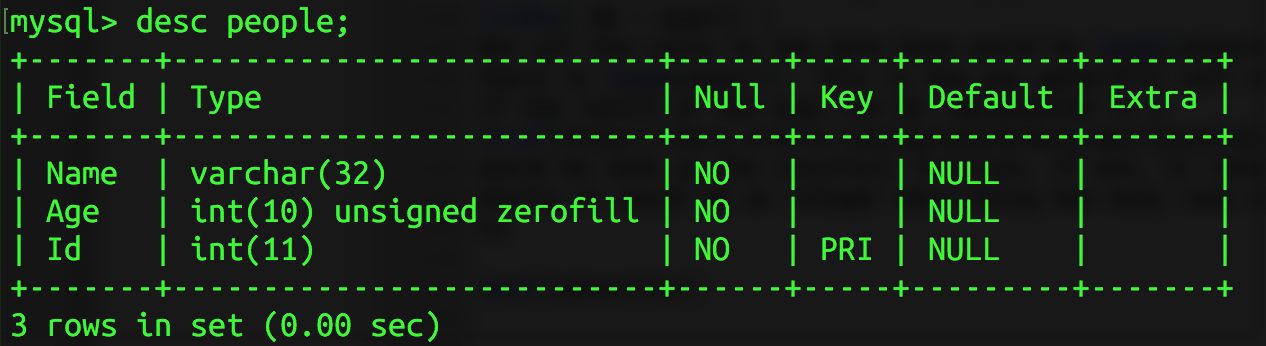
\includegraphics[width=130mm]{dbTableSchema.png}
}

The data in the table are:

\centerline{
  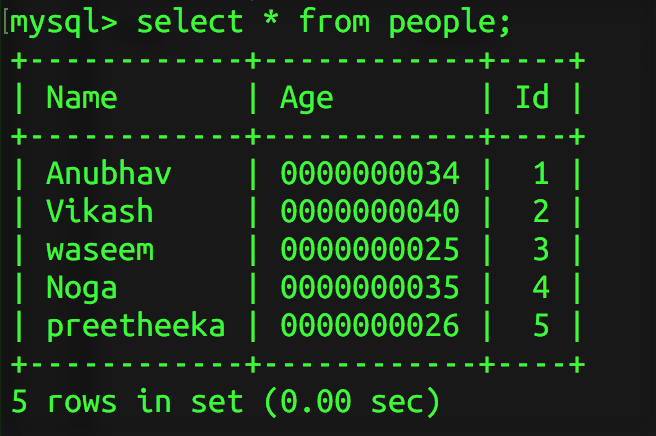
\includegraphics[width=60mm]{dbTable.png}
}


Now then, the results of the function is a data matrix:

\begin{center}\begin{minipage}{\linewidth}
\begin{lstlisting}[style=JexlStyle]
// query the database
m = db.results("localhost_noga", "select * from people")
print(m.columns)
print(m.rows) 
\end{lstlisting}
\end{minipage}\end{center}

and thus, one can do subqueries after one gets the matrix object as described
in the data matrix section.
\end{subsection}

\begin{subsection}{Executing : exec() }
\index{ db : exec() }
Not all the calls to the data base would be \emph{select} statements. For other statements,
there is \emph{exec()}. This is how you generally call a database query.
If the result of the exec can be represented in a 
\href{https://docs.oracle.com/javase/8/docs/api/java/sql/ResultSet.html}{ResultSet}, exec   
would be same as the results() function. If not, it returns the result of the query, 
mostly it would be an integer describing how many rows affected. For example,
to randomly add a row to the table, one should use :

\begin{center}\begin{minipage}{\linewidth}
\begin{lstlisting}[style=JexlStyle]
// insert into the database
insert_str = "insert into people values ('Generally Moronic', 4, 100)"
r = db.exec( "localhost_noga", insert_str )
\end{lstlisting}
\end{minipage}\end{center}

\end{subsection}
 
\end{section}










